\documentclass[tikz,border=4pt]{standalone}
\usetikzlibrary{positioning,arrows.meta,calc,backgrounds}
\usepackage[scaled=0.95]{helvet}
\renewcommand{\familydefault}{\sfdefault}
\usepackage{amssymb}
% ---------------------------------------------------------------- palette (same as all figures)
\definecolor{cD}{HTML}{2A78D6}   % data
\definecolor{cV}{HTML}{E69F00}   % visualization
\definecolor{cM}{HTML}{009E73}   % models
\definecolor{cK}{HTML}{CC79A7}   % knowledge
\definecolor{cL}{HTML}{C0392B}   % feedback loop
\definecolor{ink}{HTML}{1F2328}
\definecolor{mut}{HTML}{6E7781}
\definecolor{pan}{HTML}{F3F5F7}
\definecolor{r1}{HTML}{E69F00}\definecolor{r2}{HTML}{56B4E9}\definecolor{r3}{HTML}{009E73}
\tikzset{
  mod/.style={draw=#1, fill=#1!7, rounded corners=4pt, line width=0.9pt},
  ttl/.style={font=\bfseries\footnotesize, text=ink, anchor=north, align=center},
  sub/.style={font=\tiny, text=mut, anchor=north, align=center, text width=#1},
  chip/.style={draw=#1, fill=white, rounded corners=2pt, line width=0.6pt, font=\tiny, text=ink,
               inner sep=1.6pt, minimum height=0.34cm},
  badge/.style={circle, fill=#1, text=white, font=\bfseries\tiny, inner sep=0pt, minimum size=0.36cm},
  arr/.style={-{Stealth[length=2.4mm]}, line width=0.9pt, color=#1},
  hdr/.style={font=\bfseries\small, text=ink},
  num/.style={circle, draw=ink, line width=0.7pt, font=\bfseries\scriptsize, inner sep=0pt, minimum size=0.42cm},
}
\newcommand{\header}[3]{\node[num] at (#1,#2) {#3};}

\begin{document}
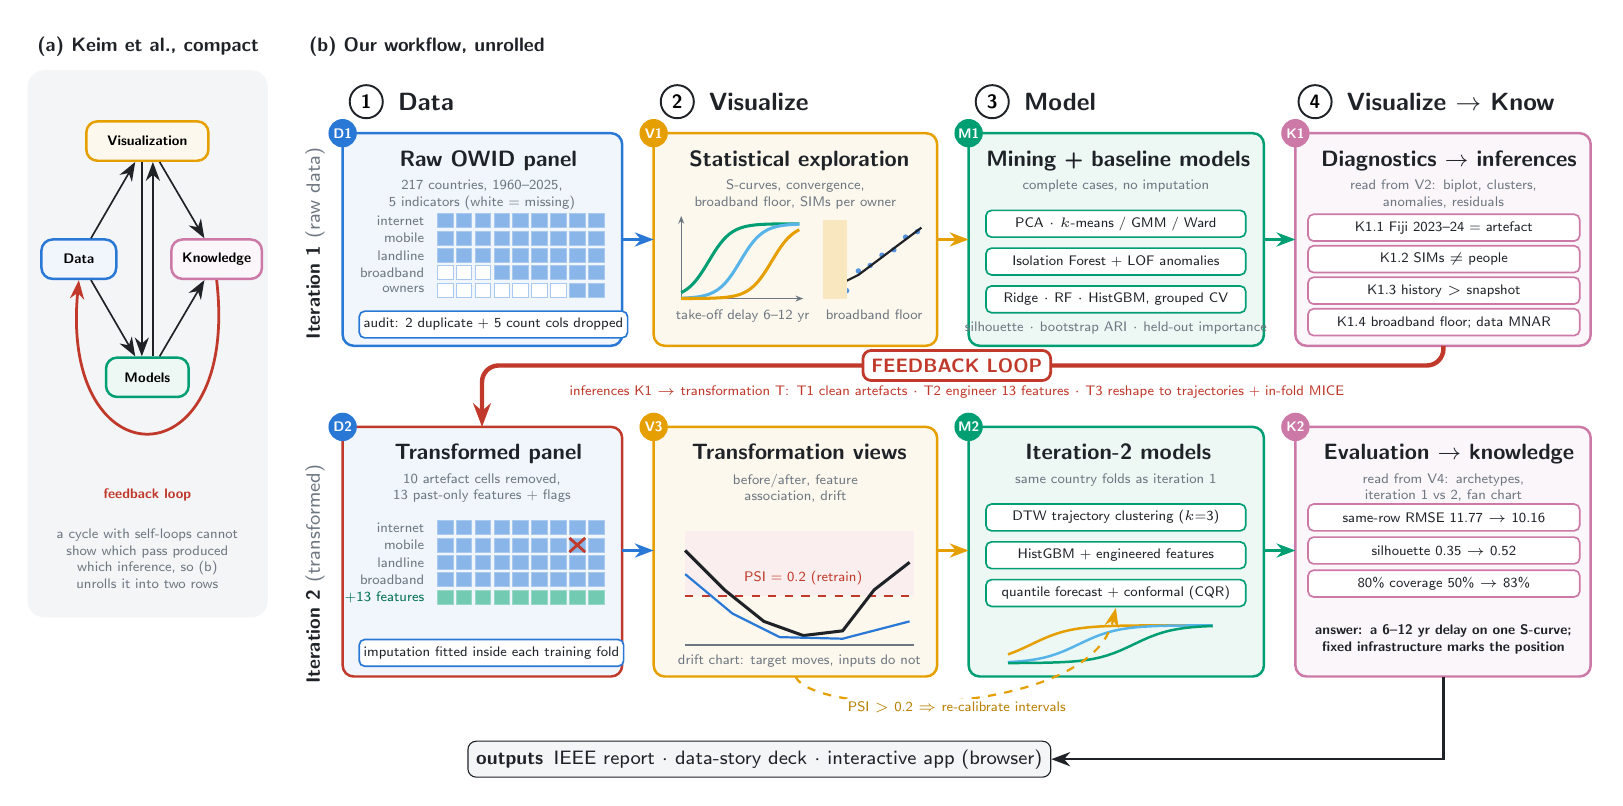
\begin{tikzpicture}[x=1cm,y=1cm]

% ================================================================ (a) compact Keim diamond
\node[font=\bfseries\scriptsize, text=ink, anchor=west] at (-0.1,9.25) {(a) Keim et al., compact};
\fill[pan, rounded corners=6pt] (-0.1,2.0) rectangle (2.95,8.95);
\node[mod=cV, minimum width=1.55cm, minimum height=0.5cm, font=\tiny\bfseries] (kv) at (1.42,8.05) {Visualization};
\node[mod=cD, minimum width=0.95cm, minimum height=0.5cm, font=\tiny\bfseries] (kd) at (0.55,6.55) {Data};
\node[mod=cK, minimum width=1.15cm, minimum height=0.5cm, font=\tiny\bfseries] (kk) at (2.3,6.55) {Knowledge};
\node[mod=cM, minimum width=1.05cm, minimum height=0.5cm, font=\tiny\bfseries] (km) at (1.42,5.05) {Models};
\foreach \a/\b in {kd/kv, kd/km, kv/kk, km/kk} \draw[arr=ink, line width=0.6pt] (\a) -- (\b);
\draw[arr=ink, line width=0.6pt] ([xshift=-2pt]kv.south) -- ([xshift=-2pt]km.north);
\draw[arr=ink, line width=0.6pt] ([xshift=2pt]km.north) -- ([xshift=2pt]kv.south);
\draw[arr=cL, line width=1pt] (kk.south) .. controls (2.6,3.7) and (0.3,3.7) .. (kd.south);
\node[font=\tiny\bfseries, text=cL] at (1.42,3.55) {feedback loop};
\node[sub=2.8cm, font=\tiny] at (1.42,3.25) {a cycle with self-loops cannot\\show which pass produced\\which inference, so (b)\\unrolls it into two rows};

% ================================================================ (b) headers
\node[font=\bfseries\scriptsize, text=ink, anchor=west] at (3.35,9.25) {(b) Our workflow, unrolled};
\header{4.2}{8.55}{1} \node[hdr, anchor=west] at (4.48,8.55) {Data};
\header{8.15}{8.55}{2} \node[hdr, anchor=west] at (8.43,8.55) {Visualize};
\header{12.15}{8.55}{3} \node[hdr, anchor=west] at (12.43,8.55) {Model};
\header{16.25}{8.55}{4} \node[hdr, anchor=west] at (16.53,8.55) {Visualize $\rightarrow$ Know};

% lane labels
\node[rotate=90, font=\bfseries\scriptsize, text=ink] at (3.55,6.75) {Iteration 1 \textcolor{mut}{\textmd{(raw data)}}};
\node[rotate=90, font=\bfseries\scriptsize, text=ink] at (3.55,2.55) {Iteration 2 \textcolor{mut}{\textmd{(transformed)}}};

% ================================================================ lane 1
% ---- D1
\draw[mod=cD] (3.9,5.45) rectangle (7.45,8.15);
\node[badge=cD] at (3.9,8.15) {D1};
\node[ttl] at (5.75,8.05) {Raw OWID panel};
\node[sub=3.4cm] at (5.67,7.68) {217 countries, 1960--2025,\\5 indicators (white = missing)};
% mini coverage grid: 5 indicators x 9 years, white = missing
\foreach \r/\miss in {0/{}, 1/{}, 2/{}, 3/{0,1,2}, 4/{0,1,2,3,4,5,6}} {
  \foreach \c in {0,...,8} {
    \def\col{cD!55}
    \foreach \m in \miss { \ifnum\c=\m \gdef\col{white} \fi }
    \fill[\col, draw=cD!40, line width=0.2pt] (5.1+\c*0.24, 6.95-\r*0.22) rectangle ++(0.2,0.18);
  }
}
\foreach \lab [count=\i from 0] in {internet, mobile, landline, broadband, owners}
  \node[font=\tiny, text=mut, anchor=east] at (5.06, 7.04-\i*0.22) {\lab};
\node[chip=cD, anchor=west] at (4.1,5.72) {audit: 2 duplicate + 5 count cols dropped};

% ---- V1
\draw[mod=cV] (7.85,5.45) rectangle (11.45,8.15);
\node[badge=cV] at (7.85,8.15) {V1};
\node[ttl] at (9.7,8.05) {Statistical exploration};
\node[sub=3.4cm] at (9.65,7.68) {S-curves, convergence,\\broadband floor, SIMs per owner};
\begin{scope}[shift={(8.2,6.05)}]
  \draw[mut, line width=0.4pt, -{Stealth[length=1mm]}] (0,0) -- (1.55,0);
  \draw[mut, line width=0.4pt, -{Stealth[length=1mm]}] (0,0) -- (0,1.05);
  \foreach \s/\cc in {0.35/r3, 0.75/r2, 1.15/r1}
    \draw[\cc, line width=1.1pt, domain=0:1.5, samples=40] plot (\x, {0.95/(1+exp(-7*(\x-\s)))});
  \node[font=\tiny, text=mut, anchor=north] at (0.78,-0.02) {take-off delay 6--12 yr};
\end{scope}
\begin{scope}[shift={(10.0,6.05)}]
  \foreach \x/\y in {0.1/0.12,0.2/0.18,0.3/0.1,0.45/0.35,0.6/0.42,0.75/0.55,0.9/0.62,1.05/0.78,1.2/0.85}
     \fill[cD!80] (\x,\y) circle (0.035);
  \draw[ink, line width=0.8pt] (0.05,0.1) -- (0.45,0.3) -- (1.25,0.9);
  \fill[cV!25] (0,0) rectangle (0.3,1.0);
  \node[font=\tiny, text=mut, anchor=north] at (0.65,-0.02) {broadband floor};
\end{scope}

% ---- M1
\draw[mod=cM] (11.85,5.45) rectangle (15.6,8.15);
\node[badge=cM] at (11.85,8.15) {M1};
\node[ttl] at (13.75,8.05) {Mining + baseline models};
\node[sub=3.6cm] at (13.72,7.68) {complete cases, no imputation};
\node[chip=cM, minimum width=3.3cm] at (13.72,7.0) {PCA $\cdot$ $k$-means / GMM / Ward};
\node[chip=cM, minimum width=3.3cm] at (13.72,6.52) {Isolation Forest + LOF anomalies};
\node[chip=cM, minimum width=3.3cm] at (13.72,6.04) {Ridge $\cdot$ RF $\cdot$ HistGBM, grouped CV};
\node[font=\tiny, text=mut] at (13.72,5.67) {silhouette $\cdot$ bootstrap ARI $\cdot$ held-out importance};

% ---- V2 / K1
\draw[mod=cK] (16.0,5.45) rectangle (19.75,8.15);
\node[badge=cK] at (16.0,8.15) {K1};
\node[ttl] at (17.95,8.05) {Diagnostics $\rightarrow$ inferences};
\node[sub=3.6cm] at (17.88,7.68) {read from V2: biplot, clusters,\\anomalies, residuals};
\foreach \t [count=\i from 0] in {K1.1 Fiji 2023--24 = artefact, K1.2 SIMs $\neq$ people, K1.3 history $>$ snapshot, {K1.4 broadband floor; data MNAR}}
  \node[chip=cK, anchor=west, minimum width=3.45cm] at (16.15,6.95-\i*0.4) {\t};

% lane-1 arrows
\draw[arr=cD] (7.45,6.8) -- (7.85,6.8);
\draw[arr=cV] (11.45,6.8) -- (11.85,6.8);
\draw[arr=cM] (15.6,6.8) -- (16.0,6.8);

% ================================================================ feedback channel
\draw[cL, line width=1.6pt, rounded corners=6pt, -{Stealth[length=3mm]}]
  (17.88,5.45) -- (17.88,5.2) -- (5.67,5.2) -- (5.67,4.42);
\node[fill=white, draw=cL, line width=1pt, rounded corners=3pt, font=\bfseries\scriptsize, text=cL,
      inner sep=3pt] at (11.7,5.2) {FEEDBACK LOOP};
\node[font=\tiny, text=cL, fill=white, inner sep=1pt] at (11.7,4.86)
  {inferences K1 $\rightarrow$ transformation T:\enspace T1 clean artefacts $\cdot$ T2 engineer 13 features $\cdot$ T3 reshape to trajectories + in-fold MICE};

% ================================================================ lane 2
% ---- D2
\draw[mod=cD, draw=cL] (3.9,1.25) rectangle (7.45,4.42);
\node[badge=cD] at (3.9,4.42) {D2};
\node[ttl] at (5.75,4.32) {Transformed panel};
\node[sub=3.4cm] at (5.67,3.95) {10 artefact cells removed,\\13 past-only features + flags};
\foreach \r in {0,...,3} \foreach \c in {0,...,8}
  \fill[cD!55, draw=cD!40, line width=0.2pt] (5.1+\c*0.24, 3.05-\r*0.22) rectangle ++(0.2,0.18);
\draw[cL, line width=1pt] (5.1+7*0.24,3.05-1*0.22) -- ++(0.2,0.18) ++(-0.2,0) -- ++(0.2,-0.18);
\foreach \lab [count=\i from 0] in {internet, mobile, landline, broadband} \node[font=\tiny, text=mut, anchor=east] at (5.06, 3.14-\i*0.22) {\lab};
\foreach \c in {0,...,8} \fill[cM!55, draw=cM!40, line width=0.2pt] (5.1+\c*0.24, 3.05-4*0.22) rectangle ++(0.2,0.18);
\node[font=\tiny, text=cM!70!black, anchor=east] at (5.06,2.26) {+13 features};
\node[chip=cD, anchor=west] at (4.1,1.55) {imputation fitted inside each training fold};

% ---- V3
\draw[mod=cV] (7.85,1.25) rectangle (11.45,4.42);
\node[badge=cV] at (7.85,4.42) {V3};
\node[ttl] at (9.7,4.32) {Transformation views};
\node[sub=3.4cm] at (9.65,3.95) {before/after, feature\\association, drift};
\begin{scope}[shift={(8.25,1.65)}]
  \fill[cL!8] (0,0.62) rectangle (2.9,1.45);
  \draw[cL, dashed, line width=0.6pt] (0,0.62) -- (2.9,0.62);
  \node[font=\tiny, text=cL, anchor=south] at (1.5,0.64) {PSI = 0.2 (retrain)};
  \draw[ink, line width=1.1pt] (0,1.2) -- (0.5,0.7) -- (1.0,0.3) -- (1.5,0.12) -- (2.0,0.18) -- (2.4,0.7) -- (2.85,1.05);
  \draw[cD, line width=0.8pt] (0,0.9) -- (0.6,0.4) -- (1.2,0.1) -- (2.0,0.08) -- (2.85,0.3);
  \draw[mut, line width=0.4pt] (0,0) -- (2.9,0);
  \node[font=\tiny, text=mut, anchor=north] at (1.45,0) {drift chart: target moves, inputs do not};
\end{scope}

% ---- M2
\draw[mod=cM] (11.85,1.25) rectangle (15.6,4.42);
\node[badge=cM] at (11.85,4.42) {M2};
\node[ttl] at (13.75,4.32) {Iteration-2 models};
\node[sub=3.6cm] at (13.72,3.95) {same country folds as iteration 1};
\node[chip=cM, minimum width=3.3cm] at (13.72,3.27) {DTW trajectory clustering ($k$=3)};
\node[chip=cM, minimum width=3.3cm] at (13.72,2.79) {HistGBM + engineered features};
\node[chip=cM, minimum width=3.3cm] at (13.72,2.31) {quantile forecast + conformal (CQR)};
\begin{scope}[shift={(12.35,1.42)}]
  \foreach \s/\cc in {0.3/r1, 0.9/r2, 1.6/r3}
    \draw[\cc, line width=0.9pt, domain=0:2.6, samples=30] plot (\x, {0.48/(1+exp(-4*(\x-\s)))});
\end{scope}

% ---- V4 / K2
\draw[mod=cK] (16.0,1.25) rectangle (19.75,4.42);
\node[badge=cK] at (16.0,4.42) {K2};
\node[ttl] at (17.95,4.32) {Evaluation $\rightarrow$ knowledge};
\node[sub=3.6cm] at (17.88,3.95) {read from V4: archetypes,\\iteration 1 vs 2, fan chart};
\node[chip=cK, anchor=west, minimum width=3.45cm] at (16.15,3.27) {same-row RMSE 11.77 $\rightarrow$ 10.16};
\node[chip=cK, anchor=west, minimum width=3.45cm] at (16.15,2.85) {silhouette 0.35 $\rightarrow$ 0.52};
\node[chip=cK, anchor=west, minimum width=3.45cm] at (16.15,2.43) {80\% coverage 50\% $\rightarrow$ 83\%};
\node[font=\tiny\bfseries, text=ink, align=center, text width=3.5cm] at (17.88,1.72)
  {answer: a 6--12 yr delay on one S-curve; fixed infrastructure marks the position};

% lane-2 arrows
\draw[arr=cD] (7.45,2.85) -- (7.85,2.85);
\draw[arr=cV] (11.45,2.85) -- (11.85,2.85);
\draw[arr=cM] (15.6,2.85) -- (16.0,2.85);
% drift triggers re-calibration (dashed, like a refresh edge)
\draw[arr=cV, dashed, line width=0.8pt] (9.65,1.25) .. controls (9.9,0.72) and (13.4,0.72) .. (13.72,2.12);
\node[font=\tiny, text=cV!80!black, fill=white, inner sep=1pt] at (11.7,0.86) {PSI $>$ 0.2 $\Rightarrow$ re-calibrate intervals};

% ================================================================ outputs bar
\draw[arr=ink, line width=0.9pt] (17.88,1.25) -- (17.88,0.2) -- (12.9,0.2);
\node[draw=ink, fill=pan, rounded corners=3pt, font=\scriptsize, text=ink, inner sep=3pt, anchor=east]
  at (12.9,0.2) {\textbf{outputs}\enspace IEEE report $\cdot$ data-story deck $\cdot$ interactive app (browser)};

\end{tikzpicture}
\end{document}
